\documentclass[spanish,12pt]{article}
\usepackage[spanish]{babel}
\usepackage[utf8]{inputenc}
\usepackage{xspace}
\usepackage{lmodern}
\usepackage{indentfirst}
\usepackage{xargs}
\usepackage{ifthen}
\usepackage{fancyhdr}
\usepackage{latexsym}
\usepackage{lastpage}
\usepackage{textcomp}
\usepackage{varwidth}
\usepackage{caratula, aed2-tad,aed2-symb,aed2-itef}
\usepackage{algorithmicx, algpseudocode, algorithm}
\usepackage{enumerate}
\usepackage{graphicx}
\usepackage{caption}
\usepackage{subcaption}
\usepackage{float}
\usepackage{anysize}
\marginsize{1.5cm}{1.5cm}{1.5cm}{1.5cm}

\begin{document}

\titulo{Informe 1}
\materia{Algoritmos y Estructuras de Datos III}
\author{Grupo  \\Alvarez Vico Jazm\'in\\Cortés Conde Titó Javier María\\Pedraza Marcelo \\ Rozenberg Uriel Jonathan}

\integrante {Jazmín Alvazer Vico}{75/15}{jazminalvarezvico@gmail.com}
\integrante {Marcelo Pedraza}{393/14}{marcelopedraza314@gmail.com}
\integrante {Uriel Jonathan Rozenberg}{838/12}{rozenberguriel@gmail.com}
\integrante {Javier María Cortés Conde Titó}{252/15}{javiercortescondetito@gmail.com}

\maketitle


\clearpage

\tableofcontents
\cleardoublepage

\section{Problema 1: Cruzando el puente}

\subsection{Inrtoducción}

En este problema, un grupo formado por arquéologos y caníbales debe cruzar un puente. El mismo sólo puede ser atravezado por dos personas a la vez, y tiene que ser cruzado con una linterna. Como el grupo sólo dispone de una linterna, siempre debe regresar alguno al lado del puente original. Además, en ningún lado del puente puede haber más caníbales que arquéologos.
Cada individuo consta de la propiedad "velocidad", un número natural que indica cuánto tiempo tarda en atravezar el puente. Si dos personas atraviezan el puente juntas, lo hacen en el tiempo más grande entre los dos.

%terminar?%

\subsection{Explicación de la solución}
Para resolver este problema, usamos la técnica de backtracking: utilizamos una función recursiva para poder probar todos los caminos posibles que no generen situaciones en las cuales hay mas caníbales que arqueólogos en algún lado del puente. Finalmente elegímos el mínimo de los subcaminos recorridos.

Para empezar, todos los casos donde ya se comienze de un lado del puente con más caníbales que arqueólogos deben devolver -1.
El caso en el cual no haya arqueologos usamos una instancia aparte que conlleva muchas condiciones booleanes. Este caso se resuelve simplemente utilizando al canibal más rápido para llevar a los demás.
 

Para los demás casos hay que analizar los cinco "movimientos"  válidos existentes para atravezar el puente: Pasar dos caníbales, pasar dos arqueólogos,pasar sólo un arqueólogo, pasar sólo un canibal o pasar un arqueólogo y un caníbal. Un movimiento es óptimo si la persona que vuelve es la más rapida de su tipo, ya que de esta manera uno minimiza la cantidad de tiempo usado en llevar de regreso la linterna, siendo que cualquier otra combinación consume más tiempo.
Para guardar la información de posiciones utilizamos una matriz de dimensión N+1xM+1 incializada en 0 y cuatro listas($N_A$ y $M_A$ para indicar quienes estan en el punto de partida y $N_B$ y$ M_B$ para el punto de llegada). cada vez que modifiquemos $N_A$ y $M_B$ se entrará en la recursión copiando M y marcando con un 1 la posicón que corresponde a ($|N_A|,|M_A|$).
Todos los resultados se guardan en una lista para poder finalmente devolver el valor minimo de la misma el cual será nuestra solución.


%creeeo que le falta%



\subsection{Pseudocódico}
\begin{algorithm}[H]{\textbf{BT}(M: Matriz nula de dim($|N_A|$+1 x $|M_A|$+1), $N_A, M_A, N_{B}, M_{B}$: Listas) }
	\begin{algorithmic}
		\If{$N_A$ == []}
			\State min $\gets$ $M_A$.min()
			\State devolver min*($|M_B|-1$)+ Sumatoria($M_B$.Sacar(min))
		\EndIf
		\State M[$|N_A$|+1][$|M_A|$+1] $\gets$1
		\State T $\gets$ []
		
		\While{i=0; i$\leq$2; i++}
			\While{j=0; j+i$\leq$2, j++}
				\If{PuedenSalir(i,j,$|N_A|,|M_A|,|N_{B}|,|M_{B}|$)}
					\State se le quitan i elementos a $N_A$ y se le agregan a $N_B$
					\State se le quitan j elementos a $M_A$ y se le agregan a $M_B$
					\State (si i,j=1 se quita el más rápido, si i,j=2 se quitan el más rápido y el más lento)
					\State t $\gets$ Max(de los elementos transferidos)
					\While{k=0; k$\leq$2; k++}
						\While{l=0; k+l$\leq$2; l++}
							\If{PuedenSalir(k,l,$|N_A|,|M_A|,|N_{B}|,|M_{B}|$) $\land$ M[$N_A$+k][$M_A$+l]=0} %verificar esto
								\State se le quitan k elementos a $N_B$ y se le agregan a $N_A$
								\State se le quitan l elementos a $M_B$ y se le agregan a $M_A$
								\State (se quitan los dos más rápidos)
								\State t=t+Max(de los elementos transferidos)+ BT(M,$N_A,M_A,N_B,M_B$)
								\State T.Agrergar(t)
							\EndIf
						\EndWhile
					\EndWhile
				\endIf
			\EndWhile
		\EndWhile
		\State devolver Min(T)

	\end{algorithmic}
\end{algorithm}


\subsection{Demostración de Correctitud}

Para mostrar la correctitud de nuestro algoritmo queremos ver dos cosas:
\begin{itemize}

	\item Recorre todos los casos: \\
Si planteamos nuestras posibilidades como una matríz, vemos que todo lo pertinente al triángulo superior entra en las podas del inicio del algoritmo. Entonces nos concentraremos en el triángulo inferior.
Al ser nuestro algoritmo una función recursiva solo terminará al llegar al caso base. Podemos ver que nuestro caso base se alcanza al obtener las dos listas inciales($N_A$, $M_A$) vacias.
Como vemos en el primer conjunto de for, creamos  tuplas (i,j) tal que generan todas las posibles formas de pasar el puente, si esa tupla puede realmente pasar por el puente, se crea una copia de las listas $N_A$, $M_A$, $N_B$, $M_B$ donde, dependiendo del i, se sacan esa cantidad de elementos la lista $N_A$ y se ponen en $N_B$ caso análogo con j y $M$'s.
Al generar todas las instancias del cruce del puente, ahora tenemos que saber todas las formas de volver el puente. De una forma similar a la explicada antes los últimos dos whiles funcionan tal que generan todas las formas de volver del puente.

	\item No hace ciclos: \\
Nuestro algoritmo no admite ciclos puesto que tiene una condición booleana sobre la matriz, la cual no permite volver a una instancia anterior en las que este el mismo conjunto de canibales y arqueologos que en los casos anteriores. La misma consiste en que solo pueden regrsar los individuos si y solo si en la posición (i,j) (donde $i= N_A$+(los arqueolos que regresn) y $j=M_A$ + (los canibales que regresan) ) hay un cero. Cada vez que se llama a la función recursivamente la posición inicial en el punto A es marcada con un 1. De esta forma es imposible realizar ciclos.

\end{itemize}




\subsection{Demostración de Complejidad}

\subsection{Experimentación}

%%%%%%%%%%%%%%%%%%%%%%%%%%%%%%%%%%%%%%%%%%%%%%%%%%%

\section{Problema 2: Problemas en el camino}

\subsection{Introducción}

En el problema enunciado, Nuestros exploradores se encuentran con una balanza de dos platos; en el de la izquierda la llave que necesitan. Para que esta sea de utilidad, al tomarla deben mantener el equilibrio de la balanza, y para realizar esto cuentan con pesas de peso igual a las potencias de tres (una pesa por potencia).
Sabiendo el peso de la llave, necesitamos saber qué pesas poner en cada plato para mantener el equilibrio original.
Podemos pensar que el lado derecho de la balanza equivale a la operación de sustracción y el izquiero a la adición. De esta forma, al agregar pesas de un lado o del otro estaríamos sumando o restando su peso.
Esto equivale a decir que, dado un entero P queremos componerlo en sumas y restas de potencias de tres distintas.

\subsection{Explicación de la solución}

Para resolver este problema, Reescribimos P en la base ternaria, y a esta secuencia la notaremos T. Entonces tenemos $P = \sum_{i=0}^{n} a_i3^i$  con $0 \leq a_i \leq 2$ y $n = log_{3}{(P)}$  entonces $T ={a_1,a_2,...,a_n}$.
Luego, tomamos en orden creciente los elementos de T. Si $a_i$ es 0, no hacemos nada. Si $a_i$ es 1, en la balanza izquierda colocamos la pesa que corresponde a $3^i$. Si $a_i =2$, colocamos una pesa de $3^i$ en la balanza derecha y sumamos 1 a $a_{(i+1)}$ (y consecuentemente, se cambian los valores posteriores de T para que continúe en base ternaria)


\subsubsection{Pseudocódigo}

Nota: Para la implementación, en vez de crear el conjunto T, vamos tomando el resto de P y dividiéndolo por 3. Entonces, el valor de la variable "rem" sería el equivalente al $a_i$ (i responde al número de iteraciones ya hechas)

\begin{algorithm}[H]{\textbf{Pesas}(Natural: P)}
	\begin{algorithmic}[1]
		\State pesa $\gets$ 1
		\While{ P $>$ 0}
		 	\State rem $\gets$ $r_3 (P)$
	    		\State P $\gets $ parte entera(P/3)
	    		\If{rem = 1}
	    			\State pesa va para la balanza izquierda    			\Else
				\If{ rem = 2}
	    				\State p$\gets$ P+1
	    				\State pesa va para la balanza derecha
				\EndIf
			\EndIf
			\State pesa $\gets$ pesa*3
		\EndWhile
	\end{algorithmic}
\end{algorithm}



\subsubsection{Demostración de Correctitud}

Primero probaremos un lema inductivamente:
$\forall n \in N$ vale que  $2*3^{n} = 3^{n+1}-3^{n}$.

Caso base:
queremos ver que $2*3^{0} = 3^{1}-3^{0}$
$2*3^0 = 2*1=2$ y $3^1-3^0= 3-1=2$ entonces $2*3^{0} = 3^{1}-3^{0}$
\\
\\
Hipótesis Inductiva:
$\forall n \in N$ vale que  $2*3^{n} = 3^{n+1}-3^{n}$
\\
\\
Paso Inductivo:
queremos ver que $\forall n \in N$ vale que  $2*3^{n+1} = 3^{n+2}-3^{n+1}$

$2*3^{n+1} = 2*3^{n}*3 $
\\
 por hipotesis inductiva: $2*3^{n}*3 = (3^{n+1}-3^{n})*3 = 3^{n+1}*3 - 3^{n}*3= 3^{n+2}-3^{n+1} $
\\
luego, como valen el caso base y el paso inductivo, entonces vale $2*3^{n} = 3^{n+1}-3^{n} \forall n \in N $

\\
Ahora para probar la correctitud del algoritmo, desarrollaremos algunos conceptos algebraicos.
Por el algoritmo de división de Euclides sabemos que podemos escribir \\  $P= q*3+ r_{3}(P)$ con $0\leq r_{3}(P) \leq 2 $. Luego, podemos escribir $q= z*3 + r_{3}(q)$, entonces $P= (z*3 + r_{3}(q))*3 +r_{3}(P)$ y así recursivamente y aplicando la distributividad de la suma podemos descomponer p en las potencias de 3. Finalmente obtendríamos $p= \sum_{i=0}^{n}{a_i 3^{i}} $ con $0 \leq a_i \leq 2$.
Ahora nuestro problema es la aparición de $a_i=2$ en la descomposición, puesto que sólo tenemos una pesa por potencia de tres. Pero por lo visto en el lema anterior, $2*3^{i}= 3^{i+1}-3^{i}$. Esto equivale a colocar la pesa $3^{i+1}$ en la balaza izquierda y la $3^{i}$ en la derecha, obteniendo el equivalente a 2 pesas $3^{1}$ en la izquierda. aplicando este proceso recursivamente, obtenemos  una descomposición de P sumando y restando sus potencias de tres sin repeticiones.


\subsubsection{Demostración de Complejidad}

El algoritmo consta de un ciclo, dentro de cada iteración, se calcula el resto y hace dos comparaciones; todas estas operaciones se ejecutan en O(1), mientras que colocar la pesa en cada balanza
es agregar un número al final de una lista. Como el modelo de lista que usamos es "List", esto se realiza en O(1).
Entonces, dentro de cada iteración solo se hacen operaciones en O(1). Esto hace que la complejidad sea la cantidad de iteraciones que hace el ciclo.

Si nos abstraemos del if, el ciclo tiene como condición que P$>$0, siendo P el valor de entrada. Como podemos observar, P es modificado dividiéndose por 3 cada iteración. Por álgebra básica sabemos que se necesesitarán como mucho $log_3(P) + 1$ iteraciones para que P sea menor a 0.
Ahora, tomando en cuenta el if hay un caso en el cual le sumamos 1 a P, lo cual afecta un poco la cuenta; volvemos a la explicación del algoritmo y tomamos el conjunto $T = {a_1,...,a_n}$ 
donde  $P = \sum_{i=0}^{n} a_i3^i$ con $0 \leq a_i \leq 2$ y $n = log_{3}{P}$, siendo el valor de rem el valor de $a_i$ en la iésima iteración.
Cuando hacemos que $P<-P+1$ nos queda que en la próxima iteración rem valdría uno más, es decir $a_{i+1}$ pasaría a valer uno más de lo que valdría en T. Ahora,  siendo estos que para todo $a_k$
valen entre 0 y 2, si $a_{i+1}$ en vez de valer 3, valdría 0 y $a_{i+2}$ valdría uno más también, y si  $a_{i+2}$ valía 2, pasaría a valer 0 y  $a_{i+3}$ valdría uno más, y así sucesivamente hasta llegar a $a_n$.
Y si resulta que también $a_n$ valía 2, entonces tendríamos un $a_{n+1}$ que pasaría a valer 1 y $a_n$ valdría 0.
Luego no hay mas casos donde $a_j$ (para $i<j<=n$) sea 2, entonces no hay más casos donde puedan volver a ocurrir este tipo de cosas, quedándonos asi, un máximo de $Log_3(P)+1$ iteraciones.

Entonces, la complejidad del algoritmo es de $\mathcal{O}(Log_{3}(P))$.
Luego, se puede probar que Log(P) es $\mathcal{O}(\sqrt(P))$


\subsection{Experimentación}
 Al momento de la experimentación inicialmente teníamos la idea de que, al no tener mejores ni peores casos a nivel de complejidad teórica, no importaba mucho que valores de P que se ingresaban, e iba a ser siempre creciente.

\subsubsection{Análisis complejidad te\'orica}
 Para el análisis de la complejidad te\'orica decidimos simplemente medir los tiempos del algoritmo aumentando el valor de entrada desde 1 hasta la cota puesta por el enunciado.
  Después de observar los resultados, encontramos una función O(Log(n)) que se asemeje aproximadamente a los resultados de las mediciones del algoritmo para poder compararlo.
  Terminamos usando la funcion $500*log_3(x)$.
  Notamos que no quedaba muy claro cómo es que las mediciones se asemejaban a $log_3(x)$. Entonces decidimos cambiar la escala:
  En vez de presentar un gráfico que muestre los ejes (X,Y) = (peso de la llave, mediciones) lo vamos a mostrar como (X,Y) = (Log(peso de la llave),Log(mediciones))

	\begin{figure}[H]
	\centering
	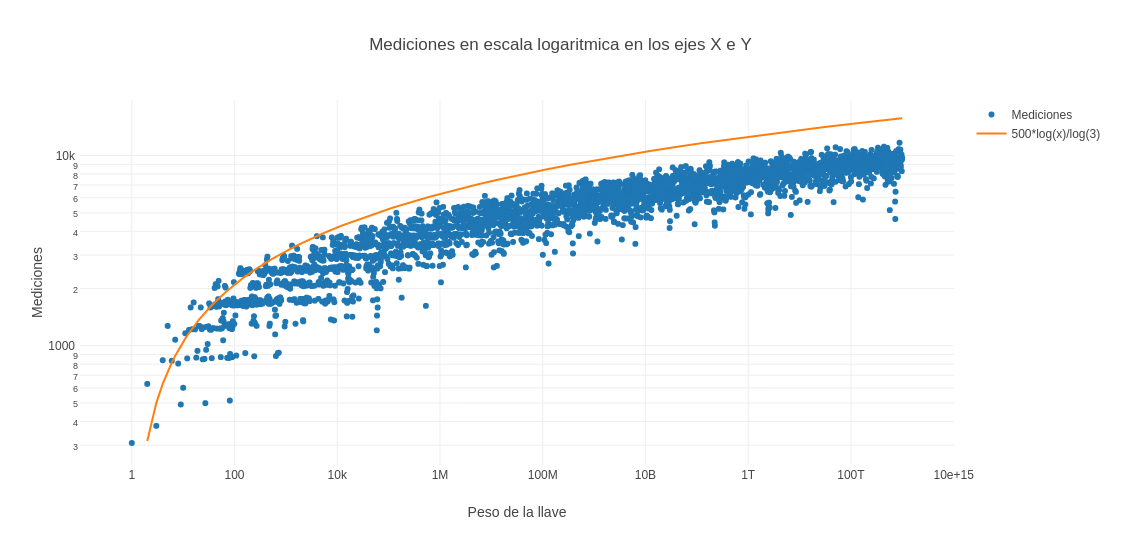
\includegraphics[width=0.8\textwidth]{punto2-mediciones}
	\caption{Mediciones de la implementaci\'on comparado con $500*log_{3}{n}$ en escala logaritmica en X e Y}
	\end{figure}



\subsubsection{Análisis}
Luego realizado el gráfico notamos que, a pesar de de que las mediciones simulaban cumplir las condiciones de la complejidad, esperábamos un comportamiento más cercano a que vaya aumentando en rectas horizontales, ya que se hacía la misma cantidad de iteraciones para cada valor del logaritmo en base 3. Pero en vez de eso éstas tenían un tipo de patrón ligeramente distinto.

\begin{figure}[H]
\centering
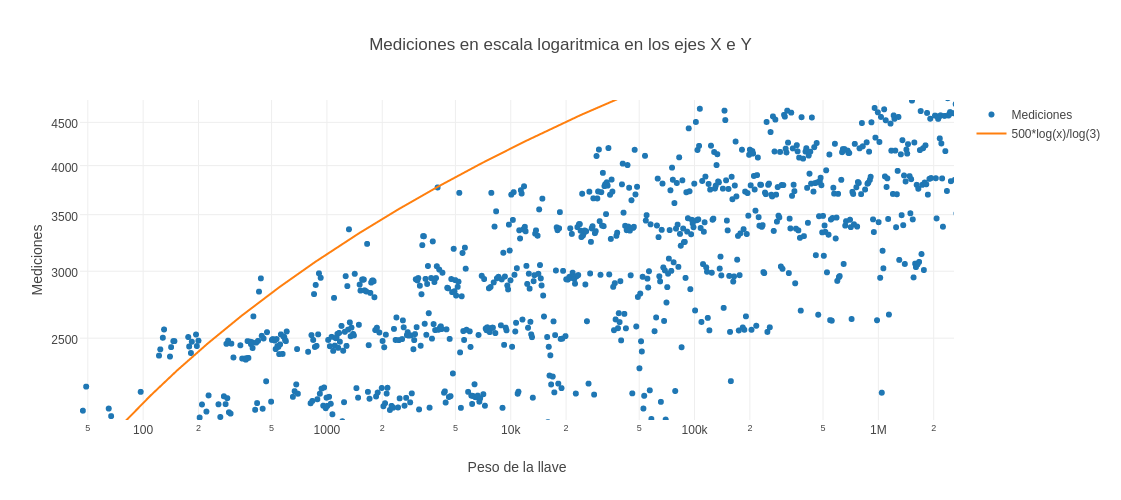
\includegraphics[width=0.8\textwidth]{punto2-zoom}
\caption{Mediciones de la implementaci\'on comparado con $500*log_{3}{n}$ zoom en escala logaritmica en X e Y }
\end{figure}
Si bien se organizaban como líneas rectas (a pesar de la escala), no se acomodaba su $"orden"$ respecto al logaritmo en base 3.
Concluímos que esto se debe a la operación "meter la pesa en una balanza", que en la implentación del problema se traduce a introducir un entero al final de una lista, lo cual termina costando $O(1)$

Para ver si esto era cierto, hicimos nuevas mediciones, tomando para los pesos  solo 3 casos: \\
-Potencias de 3: Que en la representacion ternaria, contaría solo con un 1 y puros ceros \\
-Potencias de 3 menos 1:Que en la representacion ternaria, contaría con todos 2\\
-Suma de potencias de 3:Que en la representacion ternaria, contaría con todos 1\\

y como resultado del experimento nos quedó este gráfico
\begin{figure}[H]
\centering
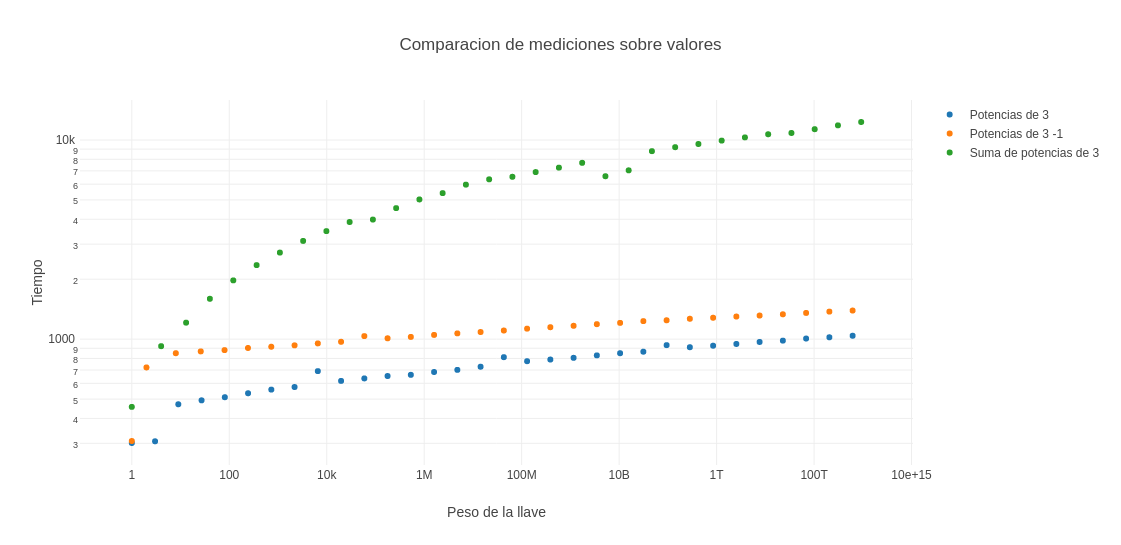
\includegraphics[width=0.4\textwidth]{punto2-comparaciones}
\caption{Comparaciones de la implementaci\'on comparando los casos en escala logarítmica en X e Y }
\end{figure}

En la imagen se puede notar que el caso de suma de potencias de 3 toma mucho más que los otros dos casos. Concluímos que esto se debe incialmente a que, en el caso de sólo potencias de 3, se hace un sólo acceso a la listar, mientras que el caso de potencias de 3 menos 1
tal como sería el resultado al problema, se pone una pesa de la potencia de 3 del lado de la llave y una pesa de tamaño 1 en el otro, teniendo así sólo 2 accesos a la lista, cosa que en la implementación esto se representa sumándole 1 luego de cada división por 3 al peso de la llave en cada iteración.

Como conclusión final a tomar en cuenta, consideramos que los mejores casos son los de potencias de 3 y los peores son los de sumas de potencias de 3.





%%%%%%%%%%%%%%%%%%%%%%%%%%%%%%%%%%%%%%%%%%%%%%%%%%%%%%%%%%%%%%%%%%%%%%%%%%%%%%%%%%%%%%%%%%%%%

\section{Problema 3: Guardando el tesoro}

\subsection{Introducción}

En este problema, los exploradores se encuentran frente a muchos tesoros que desearían poder llevarse. Para esto, cuentan con varias mochilas, cada una con una determinada capacidad de peso que puede cargar.
Los tesoros son de distintos tipos, y cada tipo tiene un peso y un valor determinado.
El objetivo es encontrar la manera óptima de llenar las mochilas para poder llevar el mayor valor posibe.

Formalmente, tenemos un conjunto de elementos que tienen como propiedad dos naturales asociados (el peso y el valor). Entonces podemos inferir que existen dos criterios de ordenamiento asociados respectivamente a estos valores.
Al mismo tiempo tenemos otro conjunto de elementos que posee como propiedad un natural asociado (capacidad).
Nuestro objetivo es seleccionar una combinación de los primeros objetos, restringida por las capacidades dadas,de modo de maximizar la sumatoria del valor de los mismos.


\subsection{Explicación de la solución}

   Inicialmente creímos que este problema podría resolverse mediante un algoritmo de BackTracking, sin embargo observamos que nunca lograríamos conseguir la complejidad pedida, puesto que este tipo de algoritmos conlleva una complejidad exponencial superior.
   Finalmente, pudimos resolverlo mediante programación dinámica. Nuestro algoritmo principal llama a dos funciones que utilizan la recursividad para poder obtener en un caso el valor óptimo, y en el otro "las mochilas llenas."
   Para facilitar el entendimiento del algoritmo introduciremos el concepto de "Hipercubo". Un hipercubo es el análogo n-dimensional de un cuadrado (n=2) o un cubo (n=3). En particular en nuestro problema tenemos un hipercubo de dimension cuatro, esta figura se denomina "teseracto", sin embargo por comodidad seguiremos llamándole hipercubo en el resto del informe.
Para poder imaginar este concepto, podríamos visualizarlo en nuestro mundo tridimencional como un vector con cubos adentro. la cantidad de cubos dependera del largo de nustra cuarta "arista".

\begin{figure}[H]
\centering
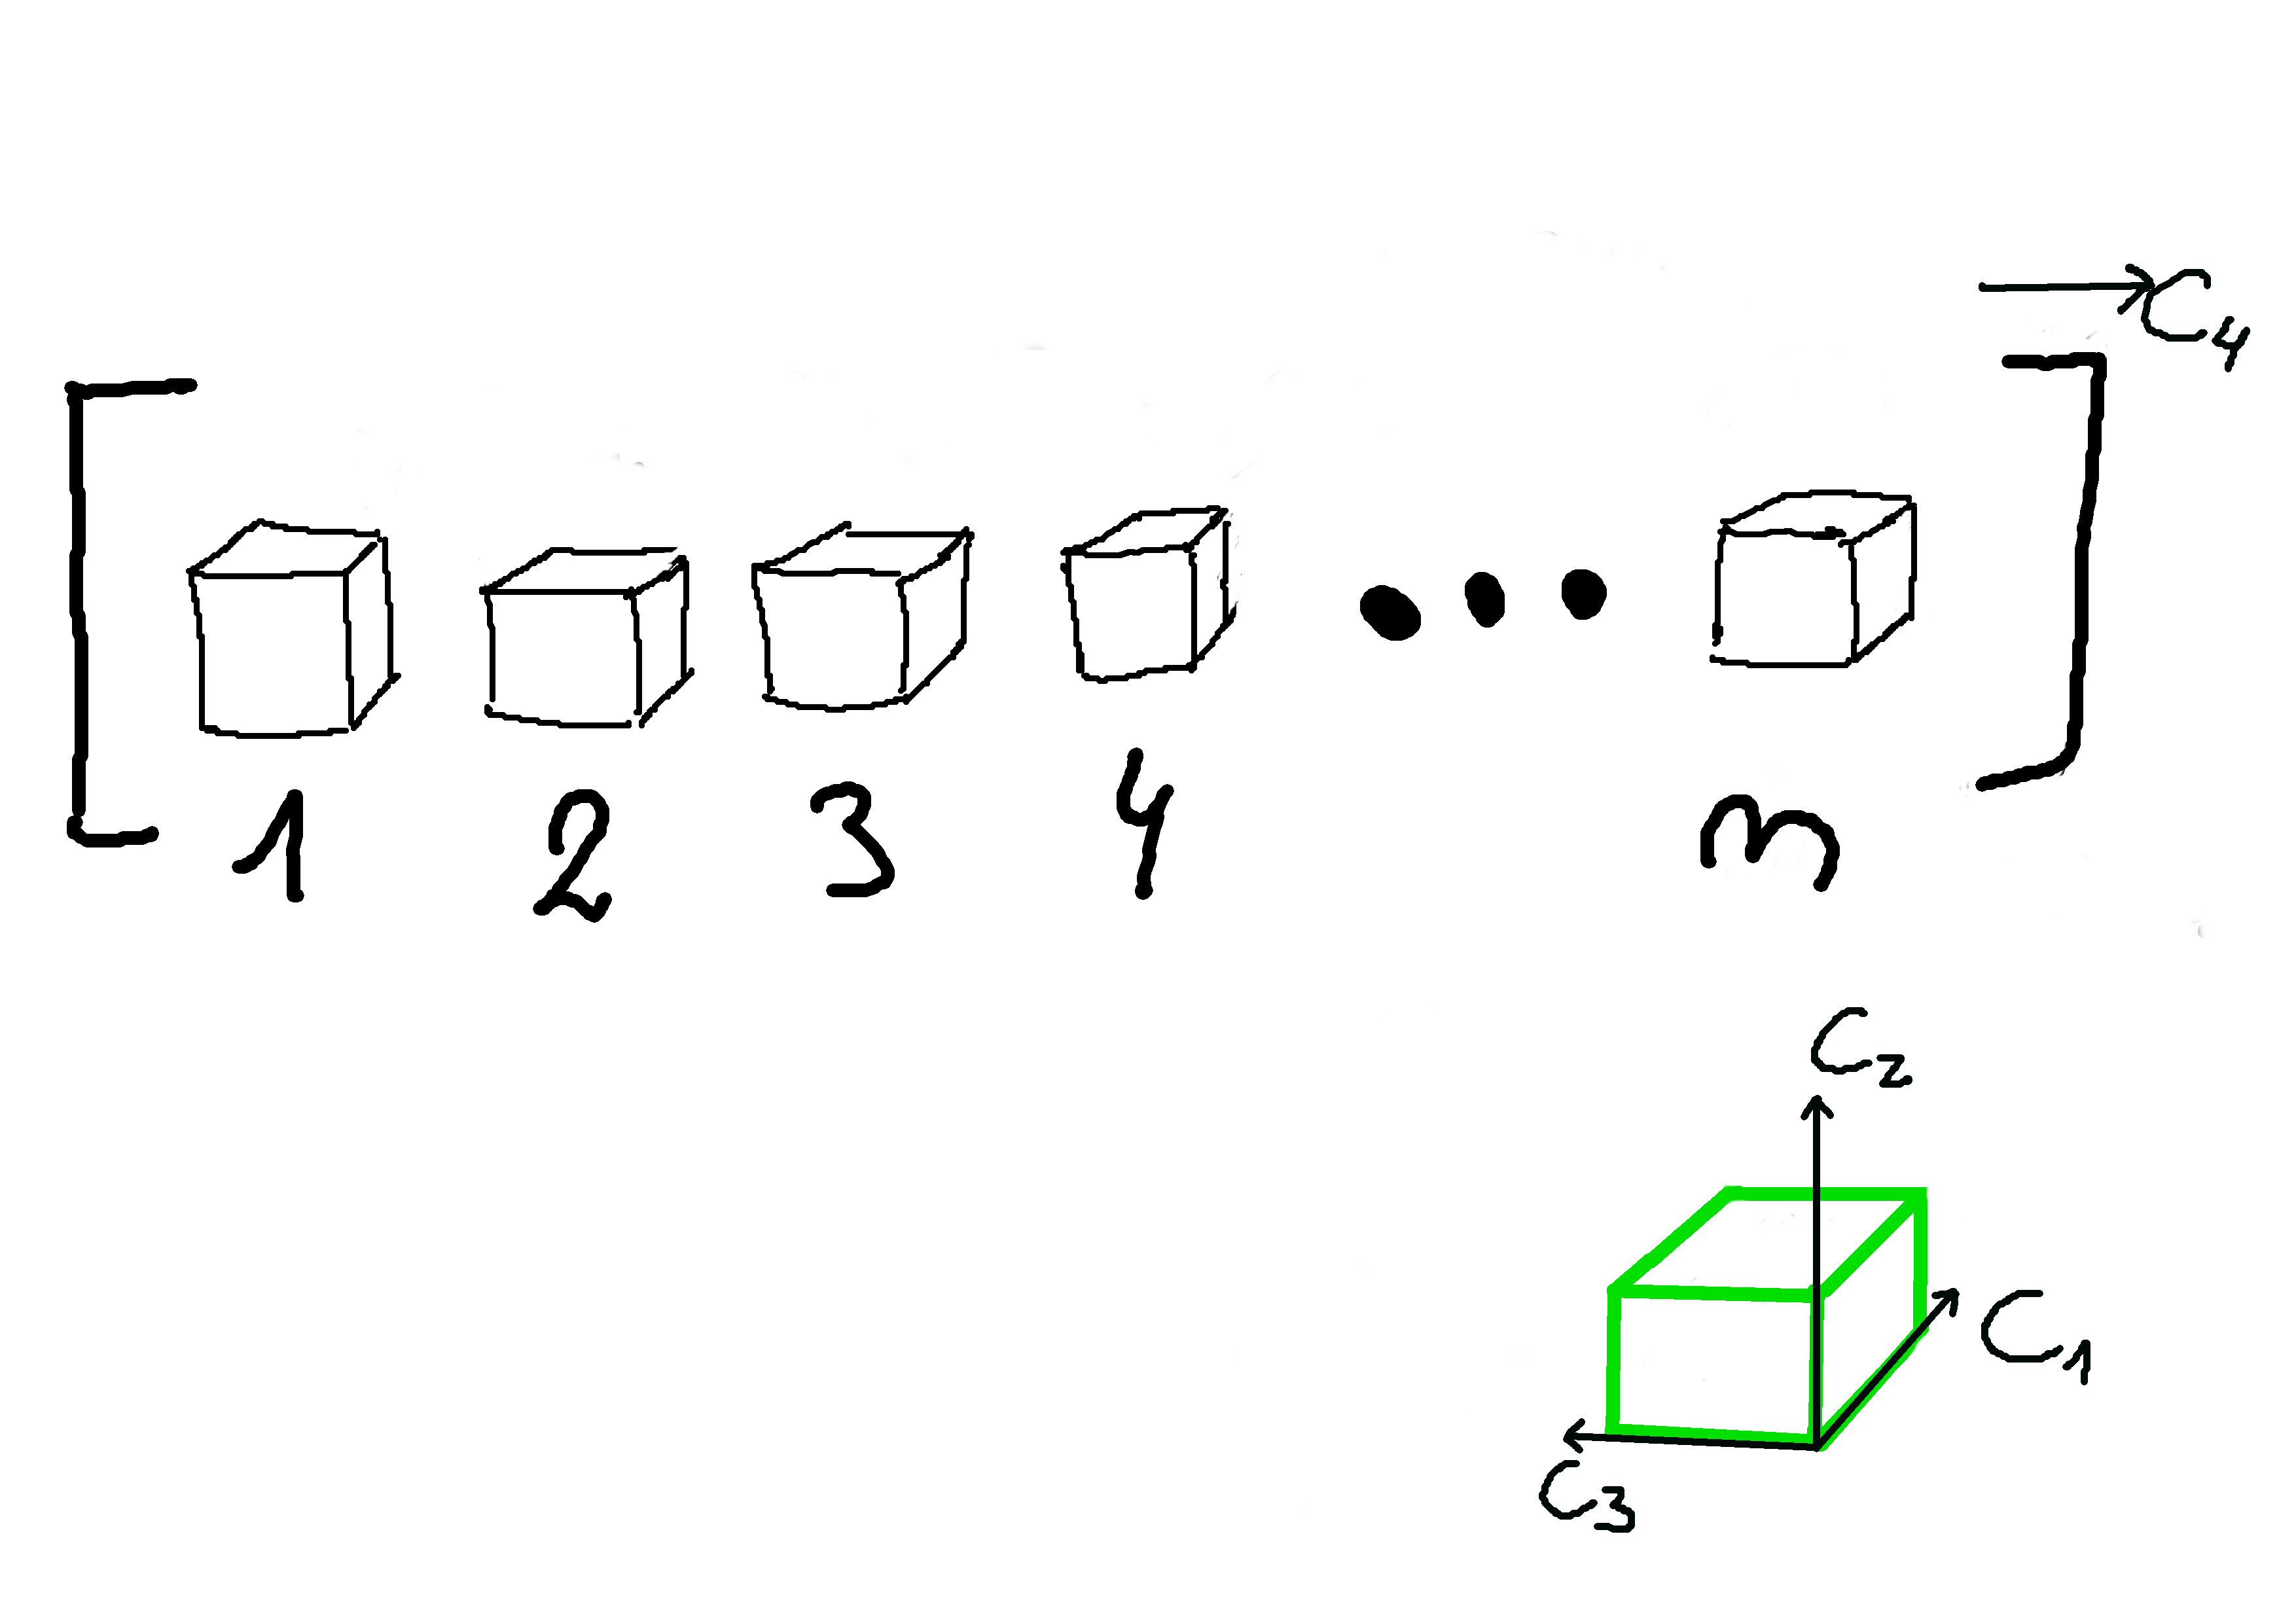
\includegraphics[width=0.4\textwidth]{hipercubo}
\caption{Imagen explicativa del concepto de hipercubo}
\end{figure}


Observación: nuestro algoritmo descarta los tesoros que tienen un peso mayor al máximo de capacidad entre las mochilas. Asumimos en el pseusocódigo que nuestra entrada cumple esa propiedad.


\subsubsection{Pseudocódigo}

\begin{algorithm}[H]{\textbf{guardandoTesoro}(mochilas: vector$<$mochila$>$, cofre: vector$<$tesoro$>$)}
	\begin{algorithmic}[1]
		%\State objXpesos $\gets$ Hipercubo() incializado en -1 \Comment (en las posiciones donde no puede haber objetos incializo en 0) %$\mathcal{O}$()
		\State objXpesos $\gets$ Hipercubo donde con todos los valores son -1 excepto en las posiciones donde no puede haber objetos que valen  0 %$\mathcal{O}$()
		\State sol$\gets$ ValorOptimo(objXpesos,cofre,cofre.size-1,capacidades de las mochilas)
		\State LlenarMochilas(objXpesos, cofre, mochila1, mochila2, mochila3)
		\State return (sol, mochilas)
	\end{algorithmic}
\end{algorithm}



\begin{algorithm}[H]{\textbf{LlenarMochilas}(objetoXpeso: hipercubo, cofre:vector$<$tesoro$>$, m1,m2,m3:mochilas)}
	\begin{algorithmic}[1]
		\State desde i= cofre.size-1 hasta i=0
			\State obj $\gets$ cofre[i]
			\State cap1 $\gets$ m1.Capacidad
			\State cap2 $\gets$ m2.Capacidad
			\State cap3 $\gets$ m3.Capacidad
			\If{$i=0$}
				\State Agregar obj en cualquier mochila en la que entre.
			\Else
				\State valM1 $\gets$ obj.valor + ValorOptimo(objetoXPeso, cofre, i,cap1-obj.peso,cap2,cap3 )
				\State valM2 $\gets$ obj.valor + ValorOptimo(objetoXPeso, cofre,i,cap1,cap2-obj.peso,cap3 )
				\State valM3 $\gets$ obj.valor + ValorOptimo(objetoXPeso, cofre,i, cap1, cap2,cap3-obj.peso )
				\State MeterEnCorrecta(valM1,valM2,valM3,m1,m2,m3,obj)
			\EndIf

	\end{algorithmic}
\end{algorithm}



%%%

\begin{algorithm}[H]{\textbf{ValorOptimo(objXpeso:hipercubo, cofre:vector$<$tesoro$>$, objeto:int, peso1: int, peso2:int, peso3:int)}}
	\begin{algorithmic}[1]
		\State  pesoObj $\gets$ cofre[objeto].peso 
		\State  pesoVal $\gets$ cofre[objeto].valor 

		\If{$peso1 < 0 \vee peso2 < 0 \vee peso3 < 0$}
			\State return $-1$ 

		\EndIf

		\If{objetoxPesos[objeto][peso1][peso2][peso3] $\neq$ -1}
			\State return objetoxPesos[objeto][peso1][peso2][peso3] 
		\EndIf
		\If{objeto $=$ 0}
			\State val $\gets$ 0 

			\If{peso1 $\ge$ pesoObj $\vee$ peso2 $\ge$ pesoObj $\vee$ peso3 $\ge$ pesoObj}
				\State val $\gets$ valorObj 

				\State objetoxPesos[objeto][peso1][peso2][peso3] $\gets$ val 
				\State return val 

			\EndIf

		\Else
			\State PosiblesSolus $\gets$ vector$<$int$>$ 
			\State sinObj $\gets$ ValorOptimo(objetoxPesos, cofre, objeto -1, peso1, peso2, peso3)
			\State PosiblesSolus.Agregar(sinObj)
			\If{peso1-pesoObj $\ge$ 0}
				\State objen1 $=$ valorObj + ValorOptimo(objetoxPesos, cofre, objeto - 1, peso1 - pesoObj, peso2, peso3)
				\State PosiblesSolus.Agrergar(objen1)
			\EndIf
			\If{peso2 - pesoObj $\ge$ 0}
				\State objen2 = valorObj + ValorOptimo(objetoxPesos, cofre, objeto - 1, peso1, peso2  - pesoObj, peso3)
				\State PosiblesSolus.Agregar(objen2)
			\EndIf
			\If{peso3-pesoObj $\ge$ 0}
				\State objen3 = valorObj + ValorOptimo(objetoxPesos, cofre, objeto - 1, peso1, peso2, peso3  - pesoObj)
				\State PosiblesSolus.Agregar(objen3)
			\EndIf
			\State valor$\gets$Max(PsiblesSolus)
			\State objetoxPesos[objeto][peso1][peso2][peso3] $\gets$ valor
			\State return valor
		\EndIf


	\end{algorithmic}
\end{algorithm}

\newpage

\subsubsection{Demostración de Correctitud}
Presentaremos la función matemática que modela nuestro problema:\\

$f(o,p_{1},p_{2},p_{3})=0 \\
f(n,p_{1},p_{2},p_{3}) = Max(V_{n}+Max(f(n-1,p_{1}-p_{n},p_{2},p_{3}), f(n-1,p_{1},p_{2}-p_{n},p_{3}), f(n-1,p_{1},p_{2},p_{3}-p_{n})),f(n-1,p_{1},p_{2},p_{3})) $
\\
Donde n representa el número de tesoro, $V_{n}$ y $P_{n}$ su valor y su peso respectivamente. $p_{1},p_{2}\ y \ p_{3}$ son las capacidades de cada mochila.

Para la demostración utilizaremos inducción global en n.
\\
\\
Caso base: queremos ver que $f(0,p_{1},p_{2},p_{3})$ resulta ser el valor máximo que se puede obtener con 0 objetos:
$f(0,p_{1},p_{2},p_{3}) = 0$ al tener 0 objetos el valor de los mismos es 0 de modo que es el máximo valor posible.
\\
\\
Hipótesis Inductiva: $\forall k<n$ vale que $f(k,p_{1},p_{2},p_{3})$ da el valor máximo que se puede obtener con k objetos.
\\
\\
Ahora queremos ver que $f(n,p_{1},p_{2},p_{3})$ da el valor óptimo para n objetos.
\\
\\
$f(n,p_{1},p_{2},p_{3}) = Max(V_{n}+Max(f(n-1,p_{1}-p_{n},p_{2},p_{3}), f(n-1,p_{1},p_{2}-p_{n},p_{3}), f(n-1,p_{1},p_{2},p_{3}-p_{n})),f(n-1,p_{1},p_{2},p_{3})) $ \\
por hipótesis inductiva (como $n-1 \leq k$ para algun k) sabemos que $f(n-1,p_{1}-p_{n},p_{2},p_{3}), f(n-1,p_{1},p_{2}-p_{n},p_{3}), f(n-1,p_{1},p_{2},p_{3}-p_{n}) y f(n-1,p_{1},p_{2},p_{3})$ son los valores óptimos que se pueden conseguir con n-1 objetos restando (o no) el peso del objeto n de modo de luego poder guardarlo en alguna mochila (o no). Utilizaremos los renombres $V_{01},V_{02},V_{03},V_{00}$ respectivamente.
Entonces tenemos: \\
$f(n,p_{1},p_{2},p_{3})= Max(V_{n}+Max(V_{01},V_{0,2},V_{03}),V_{00})$\\
Podemos ver que esta función  compara el valor óptimo de llenar las mochilas con n-1 tesoros y el tesoro n, con el valor óptimo de llenar las mochilas con n-1 tesoros sin el tesoro n (de esta forma se tiene cuenta el caso en el que el mejor valor se obtiene de poner algún objeto  de los n-1 anteriores que impide luego meter el tesoro n).\\
Como la función Max devuelve el mayor valor, el resultado sera el óptimo.
\\
Como valen P(0)..p(k) $\forall k<n$ y vale p(n) $\Rigtharrow$ vale p(n) $\forall n \in N \cup {0} $

\subsubsection{Demostración de Complejidad}

La complejidad del algoritmo GuardarTesoro es $\mathcal{O}(\prod_{i=1}^{3}K_{i} * T)$ donde $K_i$ representa la capacidad de cada mochila y T la cantidad de tesoros. Además, esta complejidad es aportada por el algoritmo ValorOptimo, entonces basaremos nuestra demostración en el mismo.

Primero haremos unas observaciones preliminares:
\begin{itemize}

	\item El volumen de un cubo es es $\prod_{i=1}^{3}A_{i}$ donde cada $A_i$ es una arista que representa el eje de la altura, el ancho o el largo. Como explicamos en la introducción gracias a nuestro modelado, sabemos que llenar una posición del cubo nos cuesta $\Theta(1)$, entonces llenarlo entero nos costará el equivalente al volumen del mismo. Podriamos visualizarlo como subdividir un cubo en cubos pequeños de dimension 1X1X1.
	\item Llenar un hipercubo con un valor determinado (como ocurre en la linea 1 de guardandoTesoro) cuesta $\mathcal{O}(\prod_{i=1}^{3}K_{i} * T)$ ya que hay T cubos para llenar.
	\item Cuando se llama a LlenarMochilas desde GuardarTesoro cuesta $\mathcal{O}(T)$ ya que en en las lineas 9,10,11 cuando se llama a ValorOptimo, el hipercubo objetoXpeso cuenta con todos lo valores ya calculados entrando en el if (linea 6) que devuelve en $\mathcal{O}(1)$ el valor.
\end{itemize}

Volviendo a la demostración, tanto en el pseudocódigo como en la función matemática podemos ver que la recursión se realiza tantas veces como la cantidad total de tesoros. Para llenar un cubo, siempre debemos recurrir al cubo anterior, uno puede pensar que esto aportaría complejidad, sin embargo, al guardar estos valores sólo construimos estos cubos una vez, y la complejidad por acceso es $\Theta(1)$.

Otra manera de verlo, es análoga a la explicación de la complejidad de llenar un cubo. Al estar llenando un hipercubo la complejidad será quivalente al hipervolumen del mismo, es decir, multiplicariamos las tres aristas anteriores por una que sería la cuarta dimensión(en este caso los tesoros).

De cualquier manera podemos concluir que la complejidad es $\mathcal{O}(\prod_{i=1}^{3}K_{i} * T)$

Ahora probemos que esta complejidad es menor a la pedida ($\mathcal{O}((\sum_{i=1}^{3}K_{i})^{3} * T)$)

$\prod_{i=1}^{3}K_{i}  = K_1*K_2*K_3$   sea $K_max = Max(K_1,K_2,K_3)$ y $K_o= K_1^3 + K_2^3 + K_3^3 - K_max^3$ entonces $K_1*K_2*K_3 < K_m^3 < K_m^3 + K_o = K_1^3+K_2^3+K_3^3 <(\sum_{i=1}^{3}K_{i})^{3}$ entonces $\prod_{i=1}^{3}K_{i}* T < \sum_{i=1}^{3}K_{i})^{3} * T $


\subsection{Experimentación}

La cota de complejidad de nuestro algoritmo es $\prod_{i=1}^{3}K_{i}* T$. Es decir que depende de la capacidad y cantidad de mochilas y la cantidad de tesoros.
En esta sección trataremos de respaldar esta cota mediante el análisis de los datos empíricos que obtuvimos a traves del testeo de nuestro algoritmo.
Con este objetivo a lo largo de los tests modificamos los inputs para observar de a una variable por vez dejando las otras constantes y así poder analizar el tiempo de ejecución en cada caso.


\subsubsection{Resultados y análisis}

En nuestro primer experimento fijamos una mochila con capacidad constante (50) y fuimos aumentando la cantidad de tesoros de a dos.
Así mismo, analizamos tres subcasos pertinentes: cuando los objetos están dados aleatoriamente (sin ninguna restricción sobre su peso), cuando el peso de los objetos se encuentra restringido a la capacidad de la mochila y cuando el peso de objetos es superior a la capacidad de la mochila.

\begin{figure}[H]
\centering
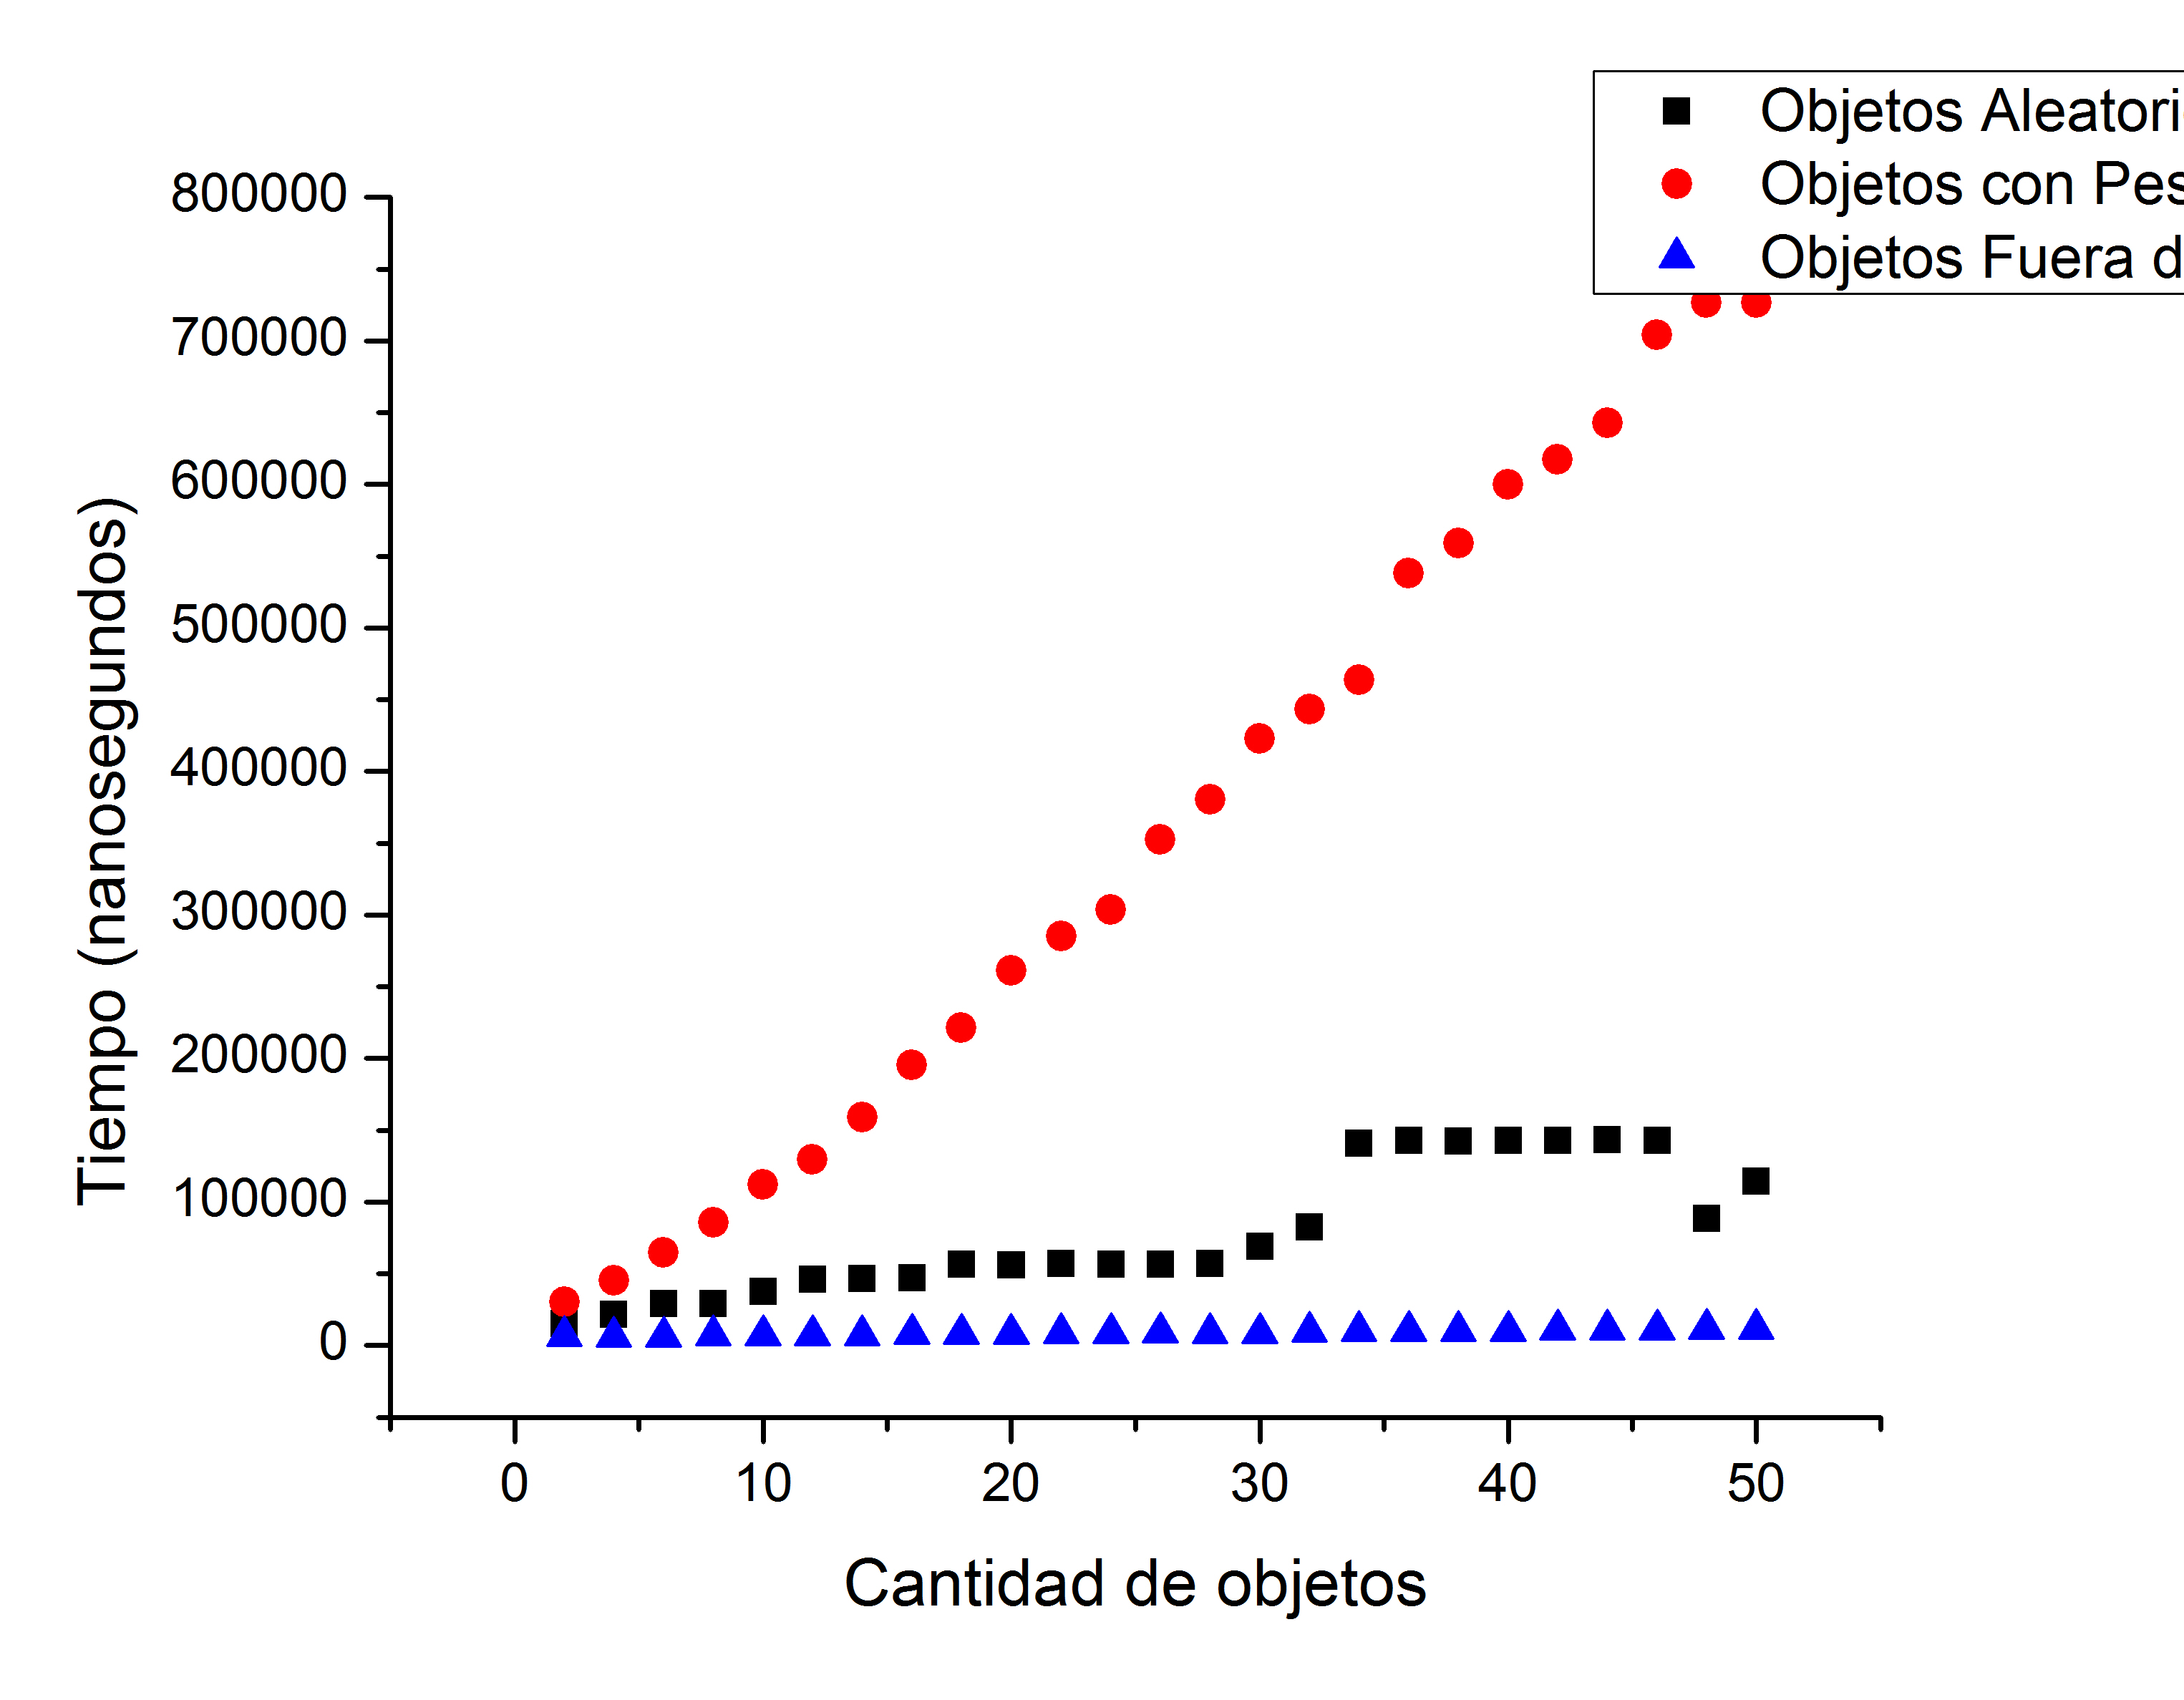
\includegraphics[width=0.6\textwidth]{comparacionObjetos}
\caption{gráfico comparativo de los tres subcasos al varias T.}
\end{figure}

<<<<<<< HEAD
En esta figura podemos observar no solo la tendencia lineal en la complejidad del algoritmo sino también la variación del crecimiento del tiempo para los distintos casos.
El hecho de que los gráficos sean lineales respaldan nuestra cota de complejidad ya que estaríamos variando el parámetro T mientras $K_1$ (la capacidad de la mochila) se mantiene constante. Estaríamos bajo la presencia de una función de tipo $Y=c*X$ con c constante.
En particular podemos destacar que en el caso de que los objetos tengan todos peso mayor a la capacidad de las mochilas, la recta tiende a ser constante y el tiempo de ejecución es casi nulo.
Podemos concluir que este sería nuestro mejor caso, y se debe al hecho de que filtramos nuestra entrada para que no se tengan en cuenta estos tesoros.
Observemos que en general lleva más tiempo obtener un resultado cuando los objetos tienen peso menor a la capacidad de la mochila.

\\
\\
Luego realizamos tests para poder ver el comportamiento del algoritmo al ir aumentando el peso de la mochila. Utilizamos un test para evaluar el comportamiento cuando los objetos son aleatorios y otro para cuando todos los tesoros tienen el peso mayor a la capacidad de la mochila.
=======
En esta figura podemos observar no solo la tendencia lineal de la complejidad del algoritmo sino también la variación de las pendientes en cada caso. Notemos que a mayor pendiente, la ejecución toma más tiempo, es decir es "más lenta".
En particular podemos destacar que en el caso de que los objetos tengan todos peso mayor a la capacidad de las mochilas, la recta tiende a ser constante.
>>>>>>> 076250449dc8b6cd7dc8911b109e73f7ced755e9

\begin{figure}[H]
\centering
\includegraphics[width=0.6\textwidth]{pesoMochila}
\caption{gráfico comparativo al variar K}
\end{figure}

Podemos observar que al tener los tesoros con peso fuera del rango de la capacidad de la mochila el tiempo se mantiene constante, prácticamente nulo igual que en el experimento anterior. Con los objetos aleatorios vemos que tiene cierta tendencia lineal como es de esperarse (ya que este caso es similar al analizando en la figura()) sin embargo algunos valores quedan distorcionados. Creemos que esto se debe a que los objetos son aleatorios.
\\
\\
Finalmente corrimos tests variando la cantidad de mochilas (todas con capacidad 50) manteniendo constantes los tesoros.

\begin{figure}[H]
\centering
\includegraphics[width=0.6\textwidth]{cantMochilas}
\caption{variación de la cantidad de mochilas.}
\end{figure}

En esta figura podemos observar el crecimiento exponencial del tiempo dependiendo de la cantidad de mochilas. Esto concuerda con el hecho de que al tener todas las variables en 50 ($T=50, K_1 =50 k_2=50, k_3=50$) al ir aumentando la cantidad de mochilas estaríamos elevando la constante 50 (con $K_1$ tenemos $K_1*T=50^2$, con $K_2$ tenemos $K_1*K_2*T=50^3, etc $). Este es el tipo de función exponencial $Y=50^X$.
\\
\\
\\






:-"Y todos estos tesoros van a ir para algun museo no?"
\\
:-"Sí,Indi... lo que digas..."



\end{document}
